\documentclass[journal,12pt,twocolumn]{IEEEtran}

\usepackage{setspace}
\usepackage{gensymb}

\singlespacing


\usepackage[cmex10]{amsmath}

\usepackage{amsthm}

\usepackage{mathrsfs}
\usepackage{txfonts}
\usepackage{stfloats}
\usepackage{bm}
\usepackage{cite}
\usepackage{cases}
\usepackage{subfig}

\usepackage{longtable}
\usepackage{multirow}

\usepackage{enumitem}
\usepackage{mathtools}
\usepackage{steinmetz}
\usepackage{tikz}
\usepackage{circuitikz}
\usepackage{verbatim}
\usepackage{tfrupee}
\usepackage[breaklinks=true]{hyperref}
\usepackage{graphicx}
\usepackage{tkz-euclide}
\usepackage{float}

\usetikzlibrary{calc,math}
\usepackage{listings}
    \usepackage{color}                                            %%
    \usepackage{array}                                            %%
    \usepackage{longtable}                                        %%
    \usepackage{calc}                                             %%
    \usepackage{multirow}                                         %%
    \usepackage{hhline}                                           %%
    \usepackage{ifthen}                                           %%
    \usepackage{lscape}     
\usepackage{multicol}
\usepackage{chngcntr}

\DeclareMathOperator*{\Res}{Res}

\renewcommand\thesection{\arabic{section}}
\renewcommand\thesubsection{\thesection.\arabic{subsection}}
\renewcommand\thesubsubsection{\thesubsection.\arabic{subsubsection}}

\renewcommand\thesectiondis{\arabic{section}}
\renewcommand\thesubsectiondis{\thesectiondis.\arabic{subsection}}
\renewcommand\thesubsubsectiondis{\thesubsectiondis.\arabic{subsubsection}}


\hyphenation{op-tical net-works semi-conduc-tor}
\def\inputGnumericTable{}                                 %%

\lstset{
%language=C,
frame=single, 
breaklines=true,
columns=fullflexible
}
\begin{document}
\newtheorem{theorem}{Theorem}[section]
\newtheorem{problem}{Problem}
\newtheorem{proposition}{Proposition}[section]
\newtheorem{lemma}{Lemma}[section]
\newtheorem{corollary}[theorem]{Corollary}
\newtheorem{example}{Example}[section]
\newtheorem{definition}[problem]{Definition}

\newcommand{\BEQA}{\begin{eqnarray}}
\newcommand{\EEQA}{\end{eqnarray}}
\newcommand{\define}{\stackrel{\triangle}{=}}
\bibliographystyle{IEEEtran}
\providecommand{\mbf}{\mathbf}
\providecommand{\pr}[1]{\ensuremath{\Pr\left(#1\right)}}
\providecommand{\qfunc}[1]{\ensuremath{Q\left(#1\right)}}
\providecommand{\sbrak}[1]{\ensuremath{{}\left[#1\right]}}
\providecommand{\lsbrak}[1]{\ensuremath{{}\left[#1\right.}}
\providecommand{\rsbrak}[1]{\ensuremath{{}\left.#1\right]}}
\providecommand{\brak}[1]{\ensuremath{\left(#1\right)}}
\providecommand{\lbrak}[1]{\ensuremath{\left(#1\right.}}
\providecommand{\rbrak}[1]{\ensuremath{\left.#1\right)}}
\providecommand{\cbrak}[1]{\ensuremath{\left\{#1\right\}}}
\providecommand{\lcbrak}[1]{\ensuremath{\left\{#1\right.}}
\providecommand{\rcbrak}[1]{\ensuremath{\left.#1\right\}}}
\theoremstyle{remark}
\newtheorem{rem}{Remark}
\newcommand{\sgn}{\mathop{\mathrm{sgn}}}
\providecommand{\abs}[1]{\vert#1\vert}
\providecommand{\res}[1]{\Res\displaylimits_{#1}} 
\providecommand{\norm}[1]{\lVert#1\rVert}
%\providecommand{\norm}[1]{\lVert#1\rVert}
\providecommand{\mtx}[1]{\mathbf{#1}}
\providecommand{\mean}[1]{E[ #1 ]}
\providecommand{\fourier}{\overset{\mathcal{F}}{ \rightleftharpoons}}
%\providecommand{\hilbert}{\overset{\mathcal{H}}{ \rightleftharpoons}}
\providecommand{\system}{\overset{\mathcal{H}}{ \longleftrightarrow}}
	%\newcommand{\solution}[2]{\textbf{Solution:}{#1}}
\newcommand{\solution}{\noindent \textbf{Solution: }}
\newcommand{\cosec}{\,\text{cosec}\,}
\providecommand{\dec}[2]{\ensuremath{\overset{#1}{\underset{#2}{\gtrless}}}}
\newcommand{\myvec}[1]{\ensuremath{\begin{pmatrix}#1\end{pmatrix}}}
\newcommand{\mydet}[1]{\ensuremath{\begin{vmatrix}#1\end{vmatrix}}}
\numberwithin{equation}{subsection}
\makeatletter
\@addtoreset{figure}{problem}
\makeatother
\let\StandardTheFigure\thefigure
\let\vec\mathbf
\renewcommand{\thefigure}{\theproblem}
\def\putbox#1#2#3{\makebox[0in][l]{\makebox[#1][l]{}\raisebox{\baselineskip}[0in][0in]{\raisebox{#2}[0in][0in]{#3}}}}
     \def\rightbox#1{\makebox[0in][r]{#1}}
     \def\centbox#1{\makebox[0in]{#1}}
     \def\topbox#1{\raisebox{-\baselineskip}[0in][0in]{#1}}
     \def\midbox#1{\raisebox{-0.5\baselineskip}[0in][0in]{#1}}
\vspace{3cm}
\title{EE3900-Assignment 5}
\author{W Vaishnavi\\AI20BTECH11025}
\maketitle
\newpage
\bigskip
\renewcommand{\thefigure}{\theenumi}
\renewcommand{\thetable}{\theenumi}
Download all latex-tikz codes from 
%
\begin{lstlisting}
https://github.com/vaishnavi-w/EE3900/blob/main/Assignment5/latex5.tex
\end{lstlisting}
and python codes from 
%
\begin{lstlisting}
https://github.com/vaishnavi-w/EE3900/blob/main/Assignment5/hyperbola.py
\end{lstlisting}
\section{Quadratic Forms Q.30}
Find the equation of a hyperbola with the vertices \myvec{0\\\pm \frac{\sqrt{11}}{2}} and foci \myvec{0\\\pm 3}
\section{Solution}
\begin{lemma}
The equation of  a conic with directrix $\vec{n}^{\top}\vec{x} = c$, eccentricity $e$ and focus $\vec{F}$ is given by 
\begin{align}
    \label{eq:conic_quad_form}
    \vec{x}^{\top}\vec{V}\vec{x}+2\vec{u}^{\top}\vec{x}+f=0
\end{align}
where     
\begin{align}
    \label{eq:conic_quad_form_v}
    \vec{V} &=\norm{\vec{n}}^2\vec{I}-e^2\vec{n}\vec{n}^{\top}, \\
    \label{eq:conic_quad_form_u}
    \vec{u} &= ce^2\vec{n}-\norm{\vec{n}}^2\vec{F}, \\
    \label{eq:conic_quad_form_f}
    f &= \norm{\vec{n}}^2\norm{\vec{F}}^2-c^2e^2
\end{align}
\end{lemma}
\begin{lemma}
    For $\abs{\vec{V}} \ne 0$, the length of the semi-major axis of the conic in \eqref{eq:conic_quad_form} is given by 
    \begin{align} 
        a = \sqrt{\frac{\vec{u}^{\top}\vec{V}^{-1}\vec{u} -f}{\lambda_1}}
        \label{eq:ab}
    \end{align}
\end{lemma}
\begin{lemma}
The eccentricity of conic \eqref{eq:conic_quad_form} is given by,
\begin{align}
    \label{eq:eccentricity} e = \sqrt{1 - \frac{\lambda_1}{\lambda_2}}
\end{align}
\end{lemma}
\begin{lemma}
For $\abs{\vec{V}} \ne 0$, given vertices $B_1,B_2$ and foci $F_1,F_2$ eccentricity of conic \eqref{eq:conic_quad_form} is given by,
\begin{align}
    \label{eq:eccentricity} e = \frac{\norm{\vec{F_1}-\vec{F_2}}}{\norm{\vec{B_1}-\vec{B_2}}}
\end{align}
\end{lemma}
\begin{proof}
Distance between the vertices is equal to the length of the major axis. That gives,
\begin{align}
    \label{eq1} \norm{\vec{B_1}-\vec{B_2}} = 2\sqrt{\frac{\vec{u}^{\top}\vec{V}^{-1}\vec{u} -f}{\lambda_1}} = 2a
\end{align}
Distance between the foci given as,
\begin{align}
    \label{eq2} \norm{\vec{F_1}-\vec{F_2}} = 2\sqrt{\frac{(\vec{u}^T\vec{V}^{-1}\vec{u}-f)(\lambda_2-\lambda_1)}{\lambda_1\lambda_2}} = 2ae
\end{align}
Dividing \eqref{eq1} and \eqref{eq2} gives $e$
\end{proof}
\begin{lemma}
Given vertex $\vec{B}$ and focus $\vec{F}$ of conic \eqref{eq:conic_quad_form}, equation of directrix is given as $\vec{n}^{\top}\brak{\vec{x} - \vec{P}} = 0$ where
\begin{align}
    \vec{P} = \vec{B} + \frac{\brak{\vec{B}-\vec{F}}}{e}\\
    \vec{n} = \vec{B}-\vec{F}
\end{align}
\end{lemma}
\begin{proof}
The directrix is perpendicular to the line joining vertex and focus. Thus normal vector for directrix is
\begin{align}
    \implies \vec{n} = \vec{B}-\vec{F}
\end{align}
$\vec{m}$ is the unit vector in the direction of $\vec{FB}$
\begin{align}
    \vec{m} = \frac{\vec{B}-\vec{F}}{\norm{\vec{B}-\vec{F}}}
\end{align}
For $\abs{\vec{V}} = 0$, the vertex is the mid-point of line joining $\vec{P}$ and $\vec{F}$
\begin{align}
    \vec{B} = \frac{\vec{P}+\vec{F}}{2}\\
    \vec{P} = 2\vec{B} + \vec{F} = \vec{B} + \frac{\brak{\vec{B}-\vec{F}}}{1}
\end{align}
For $\abs{\vec{V}} \ne 0$, the directrix passes through a point $\vec{P}$,
\begin{align}
    \vec{P} = \vec{B} + \vec{m}\frac{a\brak{1-e}}{e}
\end{align}
Substituting $a,e$ from \eqref{eq1}, \eqref{eq2} gives the lemma
\end{proof}
Solution: Let the equation of the hyperbola be
\begin{align}
     \vec{x}^{\top}\vec{V}\vec{x}+2\vec{u}^{\top}\vec{x}+f=0
\end{align}
Let $\vec{B_1}, \vec{B_2}$ be the vertices and $\vec{F_1}, \vec{F_2}$ be the foci
\begin{align}
    \norm{\vec{B_1}-\vec{B_2}} = \frac{\sqrt{11}}{2}\\
    \norm{\vec{F_1}-\vec{F_2}} = 3
\end{align}
From \eqref{eq:eccentricity} eccentricity,
\begin{align}
    e = \frac{\norm{\vec{F_1}-\vec{F_2}}}{\norm{\vec{B_1}-\vec{B_2}}} = \frac{6}{\sqrt{11}} 
\end{align}
Considering $\vec{B} = \myvec{0\\\frac{\sqrt{11}}{2}}, \vec{F} = \myvec{0\\3}$, the normal vector $\vec{n}$ of directrix
\begin{align}
    \vec{n} = \brak{\myvec{0\\\frac{\sqrt{11}}{2}}-\myvec{0\\3}} =  \myvec{0\\\frac{\sqrt{11}-6}{2}}
\end{align}
The directrix passes through the point $\vec{P}$,
\begin{align}
    \vec{P} = \myvec{0\\\frac{\sqrt{11}}{2}} +\frac{\sqrt{11}}{6}\brak{\myvec{0\\\frac{\sqrt{11}}{2}}-\myvec{0\\3}}= \myvec{0\\\frac{11}{12}}
\end{align}
Equation of the directrix can be given as
\begin{align}
    \myvec{0&\frac{\sqrt{11-6}}{2}}\brak{x - \myvec{0\\\frac{11}{12}}} = 0\\
    \implies \myvec{0&1}\vec{x} = \frac{11}{12}
\end{align}
Calculating $\vec{V}, \vec{u}$ and $f$,
\begin{align}
    \vec{V} &= 1^2\myvec{1&0\\0&1} - \brak{\frac{6}{\sqrt{11}}}^2\myvec{0\\1}\myvec{0&1}\\
    &= \myvec{1&0\\0&\frac{-25}{11}}\\
     \vec{u} &= \frac{11}{12}\brak{\frac{6}{\sqrt{11}}}^2\myvec{0\\1} - 1^2\myvec{0\\3}=\myvec{0\\0}\\
    f &= 3^2 - \brak{\frac{11}{12}\times\frac{6}{\sqrt{11}}}^2 = \frac{25}{4}
\end{align}
Equation of the hyperbola,
\begin{align}
    \vec{x}^{\top}\myvec{1&0\\0&\frac{-25}{11}}\vec{x}+\frac{25}{4}=0
\end{align}
\begin{figure}[h!]
\centering
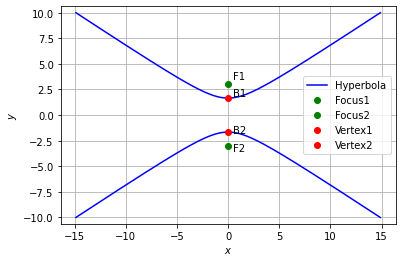
\includegraphics[width=\columnwidth]{hyperbola_plot.png}
\caption{Plot of Hyperbola}
\label{fig:hyperbola}
\end{figure}
\end{document}
